\chapter{Analysis}

Since the security of Secure Dropbox relies on the nature of different cryptography which has been justified, this chapter will mainly outline the methodologies taken in evaluating the Secure Dropbox in terms of computation performance and user experience. The methods of data collection and analyses are explained and an overview of evaluation result will also be illustrated.

\section{Evaluation Approaches}

Feedbacks of the evaluation were sought from two categories of evaluators: Dropbox users with IT background and Dropbox users without any professional understanding of IT or computer science and work in IT unrelated industries. Performance evaluation involves the efficiency of cryptography operations where network situation sometimes matters. Efficiency of cryptography involved procedures will be evaluated according to time consumed to play cryptography operation. Network environment counts when using sharing service.

Secure Dropbox was designed to fortify the security confidence of Dropbox users. It is difficult to emulate the scenario that Dropbox is under internal attack practically so the design philosophy and security provided are explained from a mathematical perspective and reasoning of its working procedure. The result data is extracted from the participants’ oral expression about their thoughts of this application. Also, the frequency of misoperations is recorded with application context to illustrate the usability of Secure Dropbox.

\section{Performance Testing}

\subsection{Testing Schema}
Performance of Secure Dropbox reflected in file encryption and decryption time consumption. The test is conducted under the hardware configuration of:

\begin{figure}[h]
        \centering
        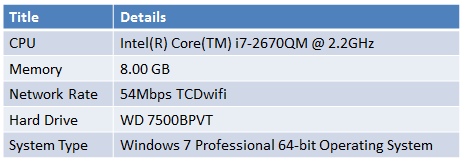
\includegraphics[width=0.7\textwidth]{figures/Testing_Environment.png}
        \caption[Testing Environment] {Testing Environment}
\end{figure}

To test the performance, several text files with different length from 1 MB to 64 MB have been created. Encryption time consumption is achieved during loading file into the Secure Dropbox procedure. The decryption time consumption is achieved from both procedures of reading local file and shared files. Downloading time is recorded during the shared file reading procedure. For values in the final performance record, each line is determined depends on average value of 100 times repeated test upon same file by performing Python scripts automatically. The results are listed as follows:

\begin{figure}[h]
        \centering
        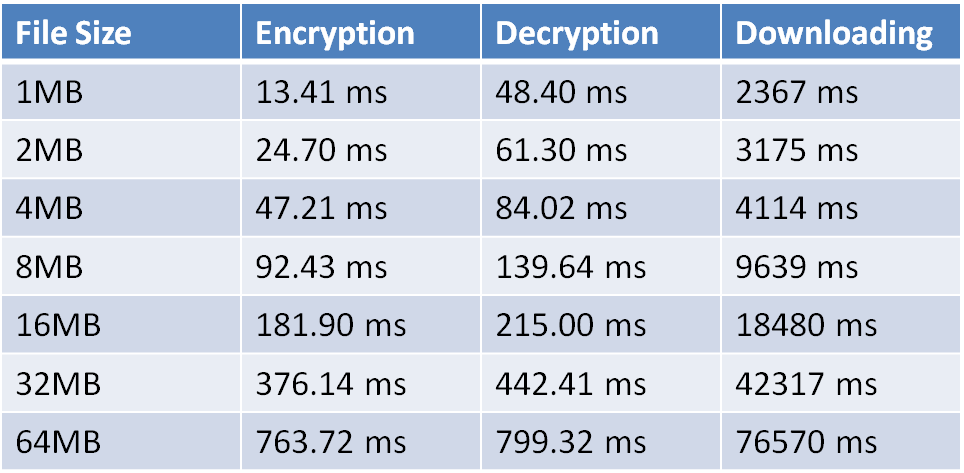
\includegraphics[width=0.7\textwidth]{figures/Secure_Dropbox_Cryptography_Performances.png}
        \caption[Secure Dropbox Cryptography Performances ] {Secure Dropbox Cryptography Performances }
\end{figure}

\subsection{Performance Evaluation}

On the basis of testing result listed above, Secure Dropbox could encrypt a 1 MB file within an average of 13.41 ms while this number comes to 763.72 ms when encrypting a 64 MB file. It could be observed that the decryption roughly costs 35 ms more than encryption no matter what the file size is. The different time consumption could be attributed to the AES decryption preparation works like unpadding the cipher and extracting initial vector. However, in comparison of the time consumption of file synchronization operation when reading shared file, the decryption time period which takes almost single-digit-percentage only could be ignored. For example, it costs more than 1 minute to download a 64 MB file but the file could be decrypted in 800 ms. The result could be concluded as satisfying concerning local file cryptography operation while the network situation becomes the bottleneck when performing large shared file reading.

\section{User Experience}

To make the user experience evaluation a generic result, Dropbox users with or without IT background are both chosen as participants. In this section the feedback received from both of them will be summarized and discussed.

\subsection{Session Procedure}

Application configuration was conducted with delivering of packed Python egg of Secure Dropbox and readme file. Assistances were given when necessary. Users tested Secure Dropbox on their PC or laptop. All the participants finished their sessions individually. During the session, participants were encouraged to finish several proposed tasks with Secure Dropbox client on their own. Participants with IT background were additionally assigned with tasks like Secure Dropbox configuring and performance evaluation. After user experience evaluation, participants were required to fill out a short questionnaire for collecting improvement comments. Users’ behavior confidence and time consumption on each task is recorded as well.

\subsection{None IT Background Users Feedback}

Most participants without IT background asked for help during Secure Dropbox configuration regarding command line operations and terminologies that involved. During testing, most of them were not skilled in command line operation style at first but got accustomed to it after several trials. Some participants forgot to press enter after finishing the OAuth procedure in the browser and instead just ignored the prompts and kept waiting in command line. All participants performed the file loading operation easily. Participant complained about that changing the source file requires another file loading operation is troublesome and easy to be forgotten. These users also commented with improvement suggestions that it would be better to make writing function integrated into the Secure Dropbox client as well so that extra file loading operations will not be essential. However they accepted the reason why this is difficult to make a generic editing interface. It was explained that different files call for different editing interface just like for ppt files Microsoft Office Power Point is required for editing. The most time consuming steps for these participants were registration and login since they were confused when typing the password to register or login but without echo on the screen. Some of them suspended the testing procedure and thought it was a program implementation problem. This is intentionally designed to imitate the way Linux does when inputting password information. Anyway it caused extremely high typo happening. Some participants proposed that there should be a contact list with permanent storage of sharing recipients’ Secure Dropbox account name in order to share a file. Also an interface to share files with a group of users should be implemented instead of performing sharing operations to each recipient one by one. One user advised that it would gain more confidence about his file’s security if Secure Dropbox could perform encryption on the same file but not on the copy in a Secure Dropbox folder. There will be only one encrypted file instance. Otherwise he had to look for other approaches to protect the plain text file. Though, he also showed his concern that he was not confident with leaving only one encrypted file instance and worried if encrypted file could not be decrypted properly. Finally, it was advised by most participants that they prefer operations in GUI or application provides a file system style user interface just like Dropbox application.

\subsection{IT Background Users Feedback}

Besides those relatively generic feedbacks, participants with IT background proposed more professional comments. Most of them advised that the file loading dialog should set file suffix filter to only display ``.txt'' files as Secure Dropbox only supports text file and other file input will be recognized as invalid operation. A few of them concerned that the OAuth procedure via browser and file loading diagram might causes availability problem in pure command line operating system like UNIX. Some participants thought an interface for querying file metadata in regard to cryptography like algorithm, key length and sharing records. Some else participants, who had been informed in advance that the Secure Dropbox disables the version control and file recovering service, advised that an operation logging system should be implemented for problem tracing in case of application errors. Some significant design defects and implementation advices have been reported during performance evaluation. Most participants thought the application crashed when reading the 64 MB shared files because there was only a blinking cursor but no any other progress indication. They advised that there should be a progress bar for time consuming operations like large file downloading or encrypting. When asked to configure the RSA key length, some participants thought the user experience should be improved. Rather than configuring by modifying the Python source code directly, an integrated configuration user interface would not only make configuration convenient and application robustness guaranteed. The configuration interface in application could play parameter checking in case of manual errors like incorrect key length is advised or illegal expressions or values for parameters. Most importantly, a fatal design defect was discovered. Encrypting a large file (i.e., 64 MB) costs less than one second while consumes far more time to synchronize file into Dropbox via Dropbox official client. However, Secure Dropbox is designed to upload file key encryption into KMS as long as the file has been encrypted. That time the file record could be queried in Secure Dropbox client but actually not in Dropbox yet. It works properly when performing a local reading since there is encrypted file instance in local file system while an exception occurs when trying to share the file because the encrypted file in Dropbox folder is not synchronized yet. It is because the “/media” interface called by Secure Dropbox to generate sharing URL cannot find the specified file which is still under synchronization. Another cryptography application design with security weakness was pointed out that once file sharing is cancelled or its URL is expired, the file encryption key should be changed in the meantime in case of someone could get the encrypted file instance and decrypt it without using shared file reading interface of Secure Dropbox client. There were implementation suggestions about integrating Secure Dropbox into file system so that it could be seamlessly used. For example, command ``sdls'' (stands for Secure Dropbox ``ls'') will be recognized as a default system command and it will directly list files loaded to Dropbox through Secure Dropbox.

\section{Discussion of Feedback}

The feedback received from the both kinds of participants with regard to security was primarily positive. They believe a client end encryption guarantees their file not accessible by Dropbox employees. Despite of those who have no concept about asymmetric cryptography, participants felt more confident to share file with Secure Dropbox in comparison of the plain text sharing by Dropbox.

Most of the criticism directed towards Secure Dropbox was concerned against the usability and design defects. Most participants thought the user interface should be improved no matter in GUI or command line for better user experience. The design flaws found during the performance test might be fatal factors to availability and security of Secure Dropbox. Future work on this application will be made based on these feedbacks.
